%%This is a very basic article template.
%%There is just one section and two subsections.
\documentclass[12pt, twoside]{article}

\usepackage[francais]{babel}
\usepackage[T1]{fontenc}
\usepackage[latin1]{inputenc}
\usepackage[left=2cm, right=3cm, top=1cm, bottom=2cm]{geometry}
\usepackage{float}
\usepackage{graphicx}
\usepackage{array}
\usepackage{multirow}
 
\begin{document}


\section*{S�ance de module du 11/09/08}

\subsection*{exercice 1: Construction de racines}
%\usepackage{graphics} is needed for \includegraphics
\begin{figure}[htp]
\begin{center}
  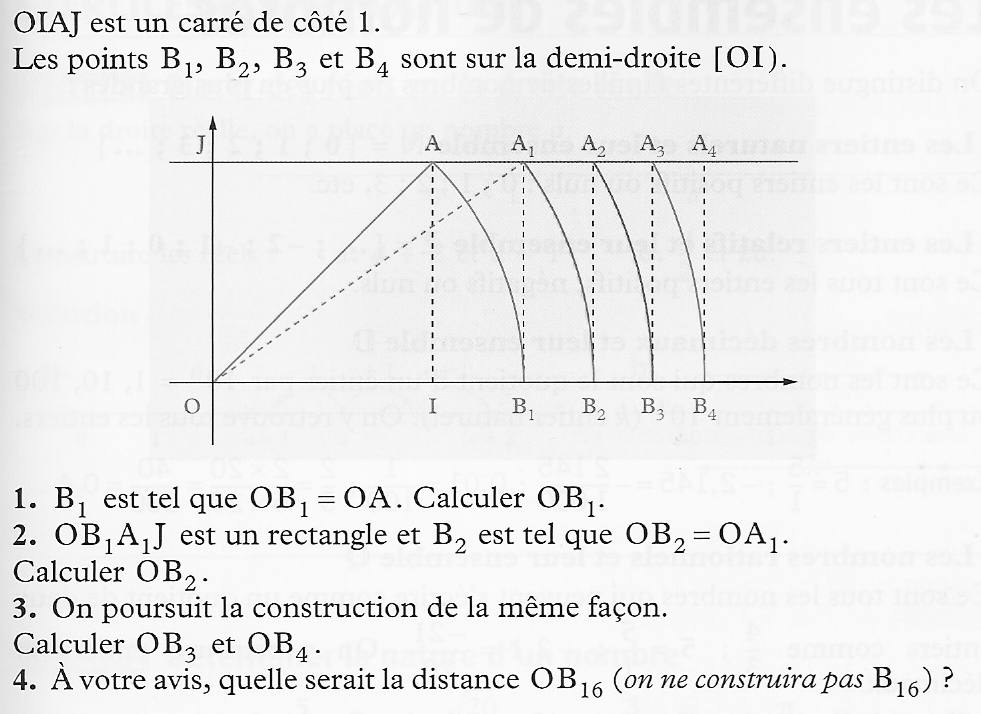
\includegraphics[width=10cm]{images/exo1.jpg}
\end{center}
\end{figure}

\subsection*{exercice 2: Calculer avec des fractions}
%\usepackage{graphics} is needed for \includegraphics
\begin{figure}[htp]
\begin{center}
  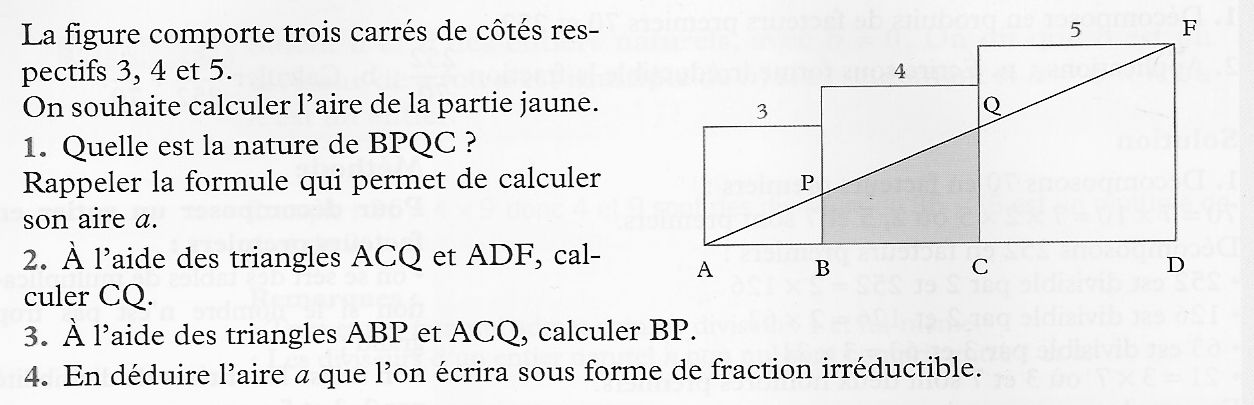
\includegraphics[width=15cm]{images/exo2.jpg}
\end{center}
\end{figure}

\subsection*{exercice 3: Le nombre d'or}
On consid�re un carr� $ABCD$ de c�t� $1$. Le point $I$ est le milieu de $[AB]$.
Le cercle de centre $I$ de rayon $IC$ coupe la demi-droite $[IB)$ en $P$.\\
\begin{tabular}{cc}
\begin{minipage}{8cm}
	\begin{enumerate}
	  \item Calculer les distances $IB$, $IC$ puis $AP$.
	  \item On note $\Phi= \frac{1+\sqrt{5}}{2}$ ($\Phi$ se lit ``phi'' et s'appelle le
	nombre d'or). Montrer que $AP*BP=AB^{2}$, en d�duire
	$\frac{AP}{AB}=\frac{AB}{BP}=\Phi$.\\ A votre avis, quelle est la nature de
	$\Phi$? (on ne demande pas la justification).
	   \item Calculer $\Phi^{2}$ et montrer que $\Phi^{2}=\Phi +1$.
\end{enumerate}
\end{minipage}
&
\begin{minipage}{7cm}
	\begin{center}
	  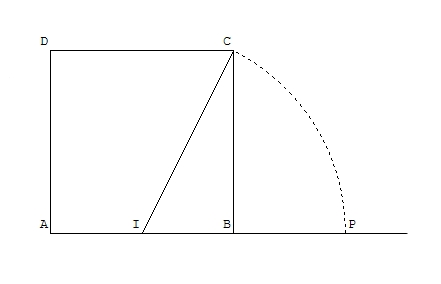
\includegraphics[width=7cm]{images/exo3.jpg}
	\end{center}
\end{minipage}
\end{tabular}

\end{document}
